\chapter{Privatsphäre ist nicht tot}
\label{les:19}

\begin{chapquote}{Lewis Carroll, \textit{Alice im Wunderland}}
Die Teilnehmer spielten alle gleichzeitig, ohne zu warten, bis sie an die Reihe
kamen; sie stritten sich andauernd; und in sehr kurzer Zeit war die Königin in
furchtbarer Laune und lief stampfend umher, wobei sie wenigstens einmal in jeder
Minute rief: \enquote{Herunter mit seinem Kopf! Herunter mit ihrem Kopf!}
\end{chapquote}

Wenn man den Experten Glauben schenkt, ist die Privatsphäre bereits seit den 80er
Jahren tot\footnote{\url{https://bit.ly/privacy-is-dead}}. Die pseudonyme
Erfindung von Bitcoin und andere Ereignisse in der jüngeren Vergangenheit zeigen,
dass dies jedoch nicht der Fall ist. Die Privatsphäre ist am Leben, auch wenn es
keineswegs einfach ist dem Überwachungsstaat zu entkommen.

Satoshi unternahm große Anstrengungen, um seine Spuren zu verwischen und seine
Identität zu verbergen. Zehn Jahre später ist noch immer unbekannt, ob Satoshi
Nakamoto eine einzelne Person, eine Gruppe von Personen, männlich, weiblich oder
eine zeitreisende KI war, die sich selbst gestartet hat, um die Welt zu
übernehmen. Verschwörungstheorien beiseite: Satoshi entschied sich als
japanischer Mann zu identifizieren, weshalb ich sein gewähltes Geschlecht
respektiere und ihn als \enquote{ihn} bezeichne.

\begin{figure}
  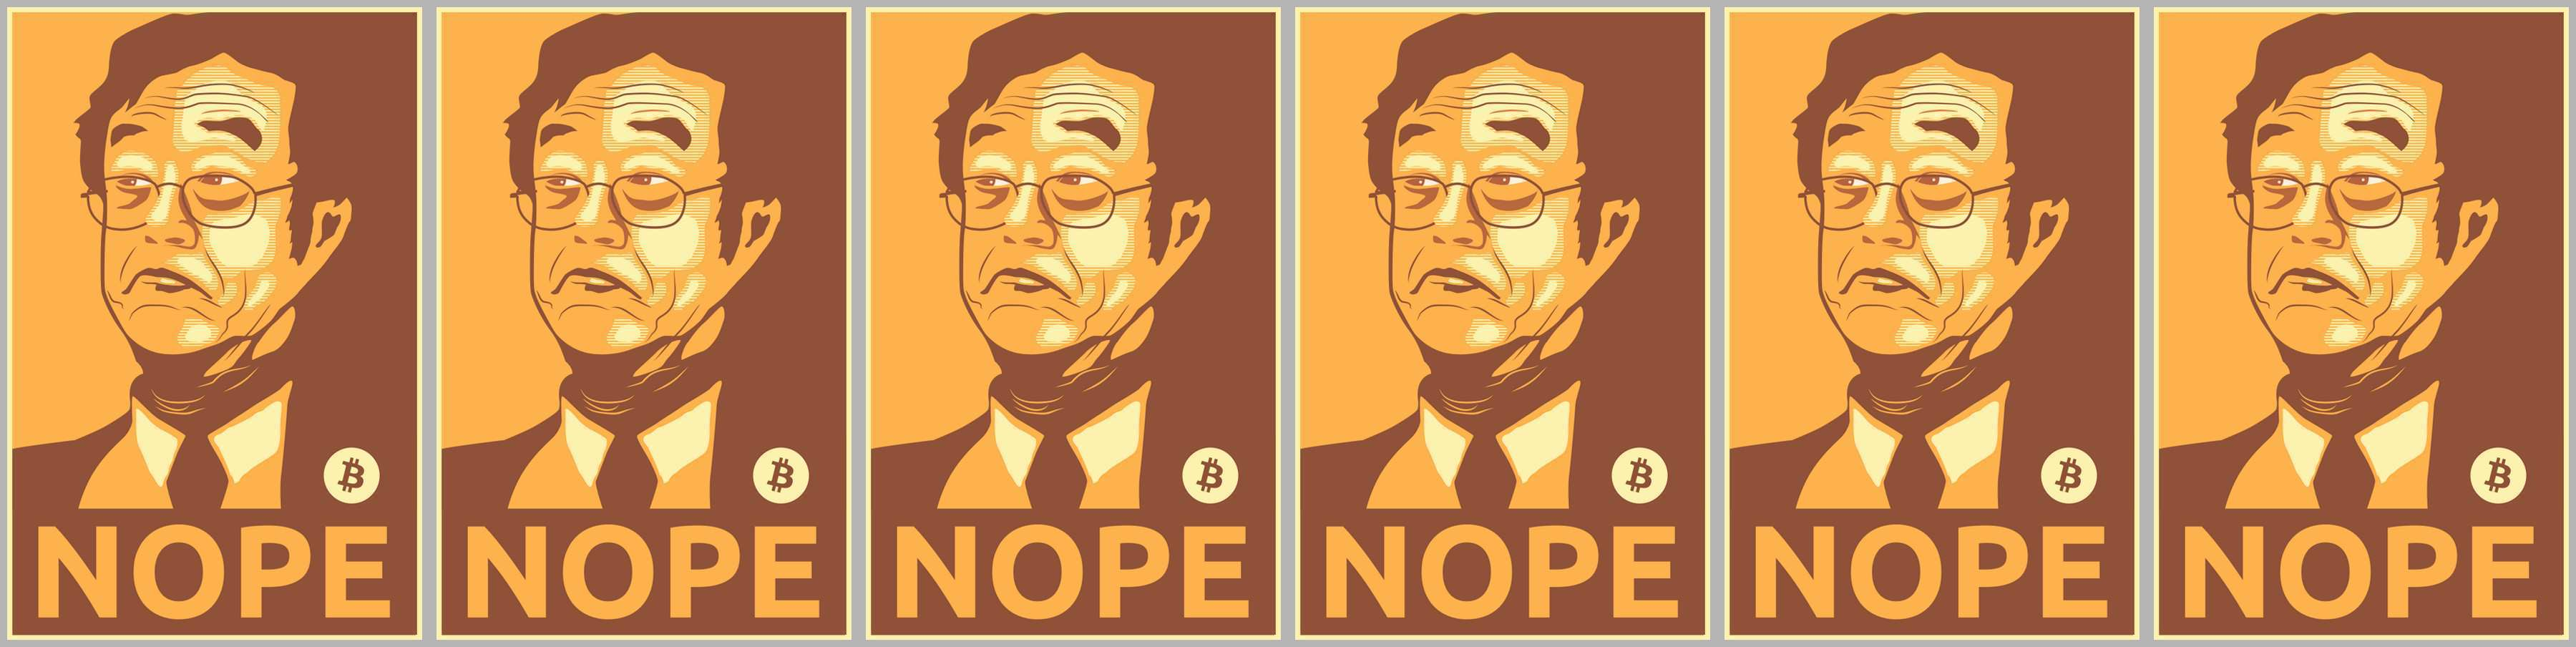
\includegraphics[width=\textwidth]{assets/images/nope.png}
  \caption{Ich bin nicht Dorian Nakamoto.}
  \label{fig:nope}
\end{figure}

\newpage

Was auch immer seine wahre Identität sein mag, Satoshi war erfolgreich dabei
diese zu verbergen. Es ist ein ermutigendes Beispiel für alle die anonym bleiben
wollen: Es ist durchaus möglich seine Privatsphäre online zu schützen.

\begin{quotation}\begin{samepage}
\enquote{Verschlüsselung funktioniert. Richtig implementierte, starke
Kryptosysteme sind eines der wenigen Dinge auf die man sich verlassen kann.}
\begin{flushright} -- Edward Snowden\footnote{Edward Snowden, in einer Antwort
auf eine Publikumsfrage \cite{snowden}}
\end{flushright}\end{samepage}\end{quotation}

Satoshi war nicht der erste pseudonyme oder anonyme Erfinder und er wird nicht
der letzte sein. Einige haben diesen pseudonymen Publikationsstil direkt
imitiert, wie Tom Elvis Yedusor von MimbleWimble~\cite{mimblewimble-origin},
andere haben fortgeschrittene mathematische Beweise veröffentlicht und sind
dabei völlig anonym geblieben~\cite{4chan-math}.

Es ist eine neue und seltsame Welt in der wir leben. Eine Welt in der Identität
optional ist, Beiträge zu Code nach Leistung beurteilt und angenommen werden und
in der Menschen frei zusammenarbeiten und handeln können. Es wird einige
Anpassungen erfordern um sich mit diesen neuen Paradigmen vertraut zu machen,
aber ich bin fest davon überzeugt, dass all dies das Potenzial, hat die Welt zum
Besseren zu verändern.

Wir alle sollten uns daran erinnern, dass die Privatsphäre ein grundlegendes
Menschenrecht ist\footnote{Allgemeine Erklärung der Menschenrechte,
\textit{Artikel 12}.~\cite{article12}}. Und solange die Menschen diese Rechte
ausüben und verteidigen, ist der Kampf um die Privatsphäre noch lange nicht
beendet.

\paragraph{Bitcoin lehrte mich, dass Privatsphäre nicht tot ist.}

% ---
%
% #### Down the Rabbit Hole
%
% - [Universal Declaration of Human Rights][fundamental human right] by the United Nations
% - [A lower bound on the length of the shortest superpattern][anonymous] by Anonymous 4chan Poster, Robin Houston, Jay Pantone, and Vince Vatter
%
% [since the 80ies]: https://books.google.com/ngrams/graph?content=privacy+is+dead&year_start=1970&year_end=2019&corpus=15&smoothing=3&share=&direct_url=t1%3B%2Cprivacy%20is%20dead%3B%2Cc0
% [time-traveling AI]: https://blockchain24-7.com/is-crypto-creator-a-time-travelling-ai/
% ["I am not Dorian Nakamoto."]: http://p2pfoundation.ning.com/forum/topics/bitcoin-open-source?commentId=2003008%3AComment%3A52186
% [MimbleWimble]: https://github.com/mimblewimble/docs/wiki/MimbleWimble-Origin
% [anonymous]: https://oeis.org/A180632/a180632.pdf
% [fundamental human right]: http://www.un.org/en/universal-declaration-human-rights/
%
% <!-- Wikipedia -->
% [alice]: https://en.wikipedia.org/wiki/Alice%27s_Adventures_in_Wonderland
% [carroll]: https://en.wikipedia.org/wiki/Lewis_Carroll
